\documentclass[a4paper,12pt]{article}

% Packages nécessaires
\usepackage[utf8]{inputenc}
\usepackage[T1]{fontenc}
\usepackage[french]{babel}
\usepackage{graphicx} % Pour inclure des images
\usepackage{caption} % Pour personnaliser les légendes
\usepackage{array} % Pour les tableaux
\usepackage{mathpazo} %police pas mal
%\usepackage{lmodern} % Police Latin Modern
\usepackage{amsmath} % Pour les formules mathématiques
\usepackage{geometry} % Pour ajuster les marges
\usepackage{fancyhdr} % Pour personnaliser les en-têtes et pieds de page
\usepackage{tikz} % Pour les images en arrière-plan
\usepackage{lipsum} % Pour générer du texte d'exemple
\geometry{top=4cm, bottom=2.5cm, left=2.5cm, right=2.5cm, headheight=2cm, headsep=1cm}
%\renewcommand{\thetable}{Tableau \arabic{table}}


% Début du document
\begin{document}

% Page de titre
\begin{titlepage}
    \begin{minipage}[t]{0.4\textwidth}
        
\includegraphics[width=\textwidth]{media/logo-enit-2454399073.png} \\[1cm] % Logo de l'établissement
    \end{minipage}
    \centering
    \vspace*{2cm}
    \begin{tikzpicture}[remember picture, overlay]
        \node[opacity=0.2, anchor=south] at (current page.south) {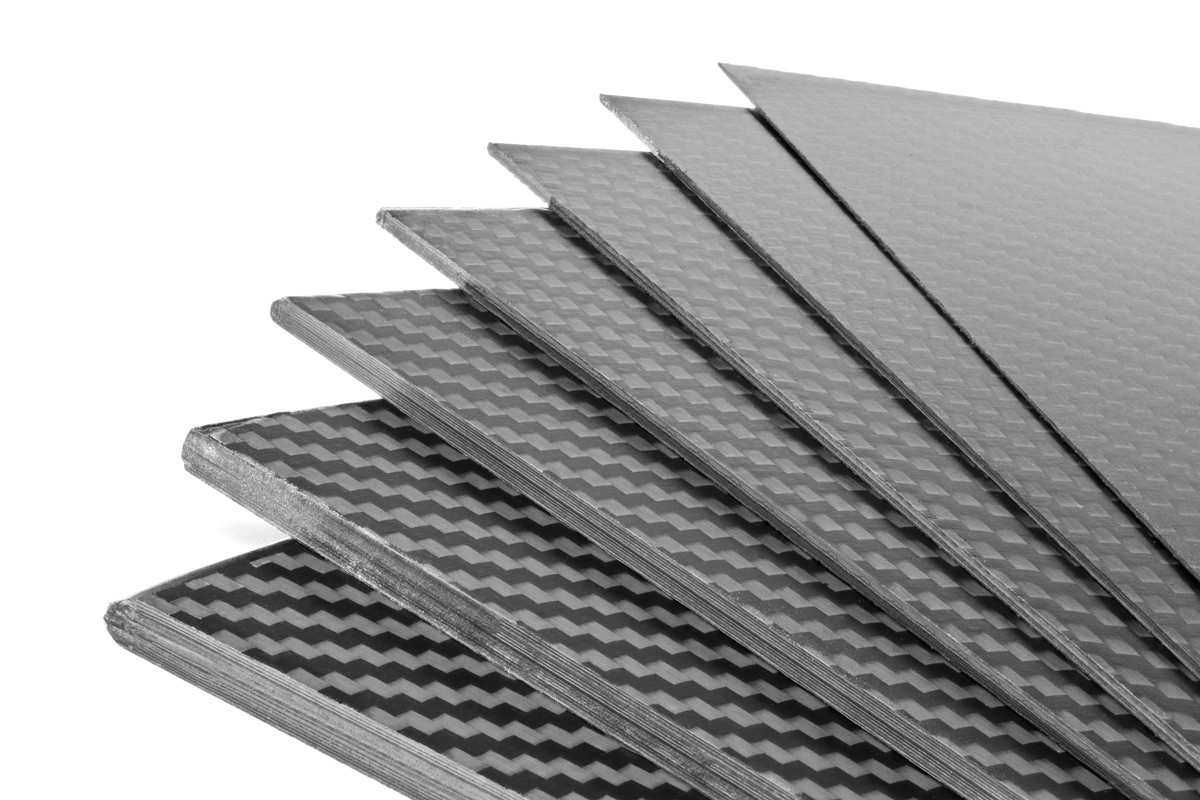
\includegraphics[width=1\paperwidth]{media/plaquecarbonne.jpg}}; % Image d'arrière-plan
    \end{tikzpicture}
    
    {\scshape \Large Rapport de TP} \\[0.5cm] % Type de document
    {\Huge \textbf{Structures composites}} \\[1.5cm] % Titre du TP
    {\large \textbf{Killian RENOU \\ William GUILBERT}} \\[0.5cm] % Noms des auteurs
    {\large \textbf{Date : 12/04/2025}} \\[0.5cm] % Date
    {\large \textbf{ENIT - École Nationale d'Ingénieurs de Tarbes}} \\[0.5cm] % Établissement
    \vfill
    {\large \textbf{Encadrant : Christian GARNIER}} % Nom de l'encadrant
\end{titlepage}


% Configuration des en-têtes et pieds de page
\pagestyle{fancy}
\fancyhf{} % Efface les en-têtes et pieds de page par défaut
\fancyhead[L]{
\includegraphics[width=3cm]{media/logo-enit-2454399073.png}} % Logo à gauche
\fancyhead[C]{\textbf{Rapport de TP Structures Composites}} % Titre au centre
\fancyhead[R]{\textbf{ Killian RENOU  \\ William GUILBERT}} % Noms à droite, l'un sous l'autre
\fancyfoot[R]{\thepage} % Numéro de page centré en pied de page
\renewcommand{\headrulewidth}{0.4pt} % Ligne noire sous l'en-tête

% Table des matières
\tableofcontents
\newpage

% Introduction
\section{Introduction}
Dans cette section, introduisez le sujet du TP, les objectifs et le contexte.

% Plaque 1
\section{Plaque 4 plis sans symétrie mirroir sous chargement mécanique}
\subsection{Hypothèses nécessaires à la mise en place du modèle numérique}
\begin{table}[h!]
	\centering
	\renewcommand{\arraystretch}{1.2} % Augmente l'interligne des lignes du tableau
	\begin{tabular}{r|p{10cm}}
		Formulation & Structure, coque 2D     \\
		Espace de modélisation & 3D (Courbure induite par l'asymétrie de la structure soumise à de la traction)  \\
		\hline
		Géométrie   & Plaque de William (L=???mm, l=???mm), plaque de Killian (L=400mm, l=400mm)\\
		\hline
		Matériau   & Pli composite UD, Loi de comportement: linéaire élastique isotrope transverse (E\textsubscript{l} = 38 Gpa, E\textsubscript{t} = 9 Gpa, $\nu$\textsubscript{lt} = 0,32, G\textsubscript{lt} = 3,6 Gpa)\\
		\hline
		Comportement de structure   & Coque 2D composite, Lay-Up \\
		\hline
		Type d'analyse   & Statique, temps d'analyse: 1s\\
		\hline
		Cas de chargement   & \begin{tabular}[t]{@{}p{10cm}}
			Pas de conditions initiales ni de conditions aux limites \\
			Force linéique N\textsubscript{xx} (l.a: l1+l2, direction x, sens: +x (l1), -x (l2), Amplitude = 1000 N.mm\textsuperscript{-1}) , \\
			Force linéique N\textsubscript{yy} (L.a: L1+L2, direction y, sens: +y (L1), -y (L2), Amplitude = 500 N.mm\textsuperscript{-1}) , \\
			Force linéique N\textsubscript{xy} (L.a: L1+L2, direction x, sens: +x (L1), -x (L2), Amplitude = 250 N.mm\textsuperscript{-1}) , \\
			Force linéique N\textsubscript{xy} (l.a: l1+l2, direction y, sens: +y (l1), -y (l2), Amplitude = 250 N.mm\textsuperscript{-1}) , \\
		\end{tabular} \\
		\hline
		Maillage   & \begin{tabular}[t]{@{}p{10cm}}
			Famille d'éléments: coque \\
			Bibliothèque d'éléments: standard \\
			Forme déléments: quadrilatère \\
			Nombre de nœuds par élément: 4 (interpolation linéaire)\\
			Nombre de DDL par noeud: 5 \\
			Intégration réduite\\
			Taille d'éléments optimisée\\

		\end{tabular} \\
		\hline
		Donnée de sortie   & U, $\sigma$, $\varepsilon$, Critère de rupture \\
	\end{tabular}
	\caption{Hypothèses pour la plaque 1}
	\label{Tableau 1: Hypothèses pour la plaque 1}
\end{table}

\subsection{Mise en place du modèle numérique sous Abaqus}
Les hypothèses nous ont permis de mettre en place le modèle numérique de la plaque 1 en considérant l'empilement suivant:

\begin{table}[h!]
	\renewcommand{\arraystretch}{1.2} % Augmente l'interligne des lignes du tableau
	\centering
	\begin{tabular}{c|c|c}
		\textbf{N° pli} & \textbf{Orientation (°)} & \textbf{Epaisseur (mm)} \\
		\hline
		4         & 15              & 1,5            \\
		3          & -30              & 1            \\
		2          & -15              & 1,5           \\
		1         & 30             & 1           \\
	\end{tabular}
	\caption{Lay-up de la plaque 1 asymétrique}
	\label{tab:exemple_tableau}
\end{table}

\begin{figure}[h!]
	\centering
	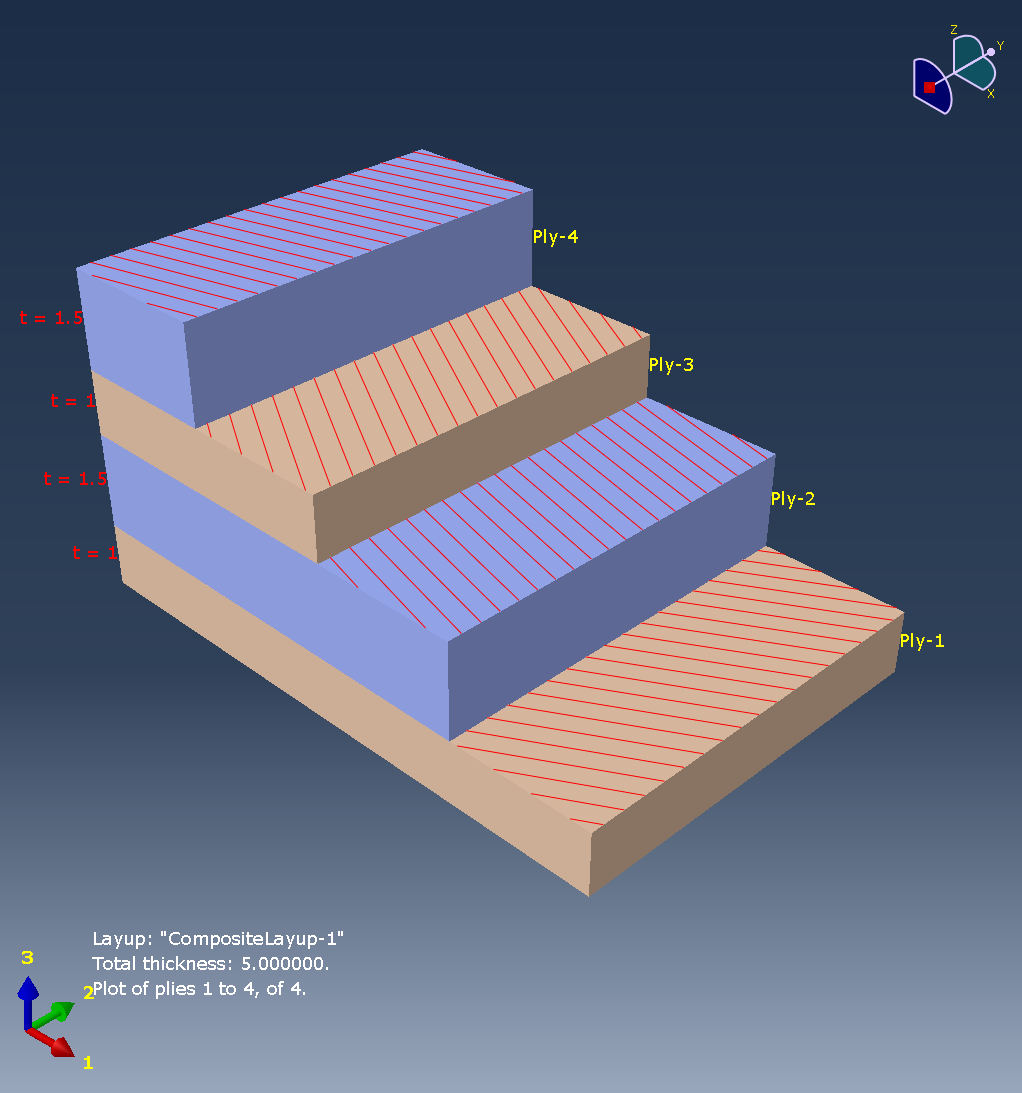
\includegraphics[width=0.5\textwidth]{media/K_P1_layout_12042025.png} % Remplacez par le chemin de votre image
	\caption{Lay-up de la plaque 1 visualisé sous Abaqus.}
	\label{fig:exemple_image}
\end{figure}

\section{Résultats obtenus sous Abaqus}

%résultats de la plaque 1, couche 1
\begin{figure}[h!]
	\centering
	\begin{minipage}[t][0.3\textheight]{0.495\textwidth}
		\centering
		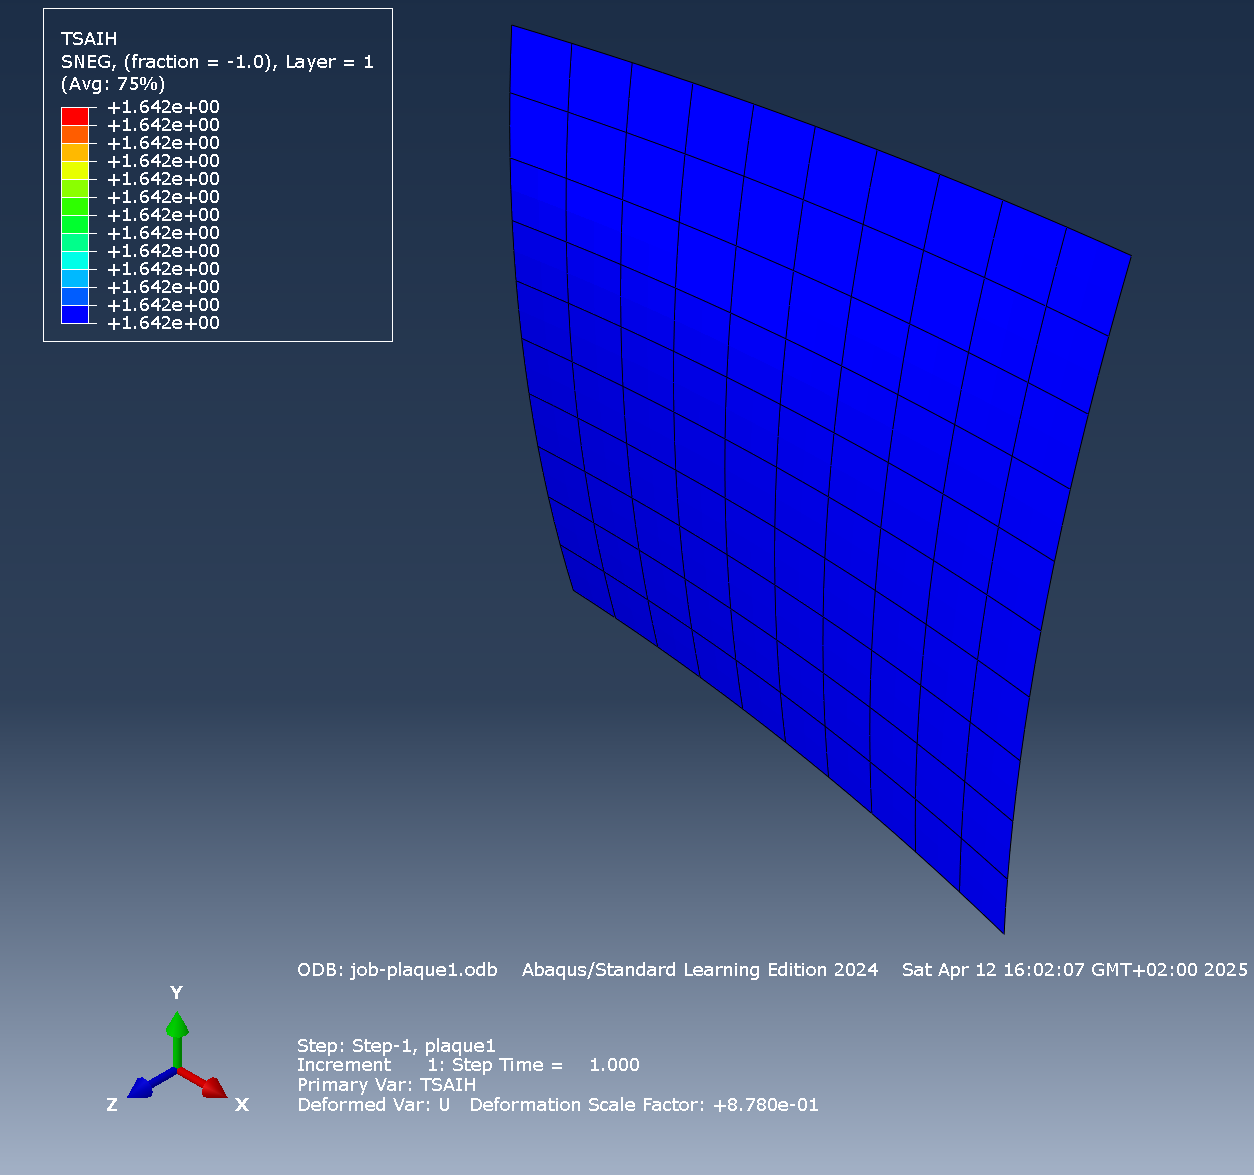
\includegraphics[width=\textwidth]{media/K_P1_L1_12042025.png} % Remplacez par le chemin de votre première image
		\caption{Couche 1, plaque carrée (Killian)}
		\label{fig:image1}
	\end{minipage}
	\hfill
	\begin{minipage}[t][0.3\textheight]{0.495\textwidth}
		\centering
		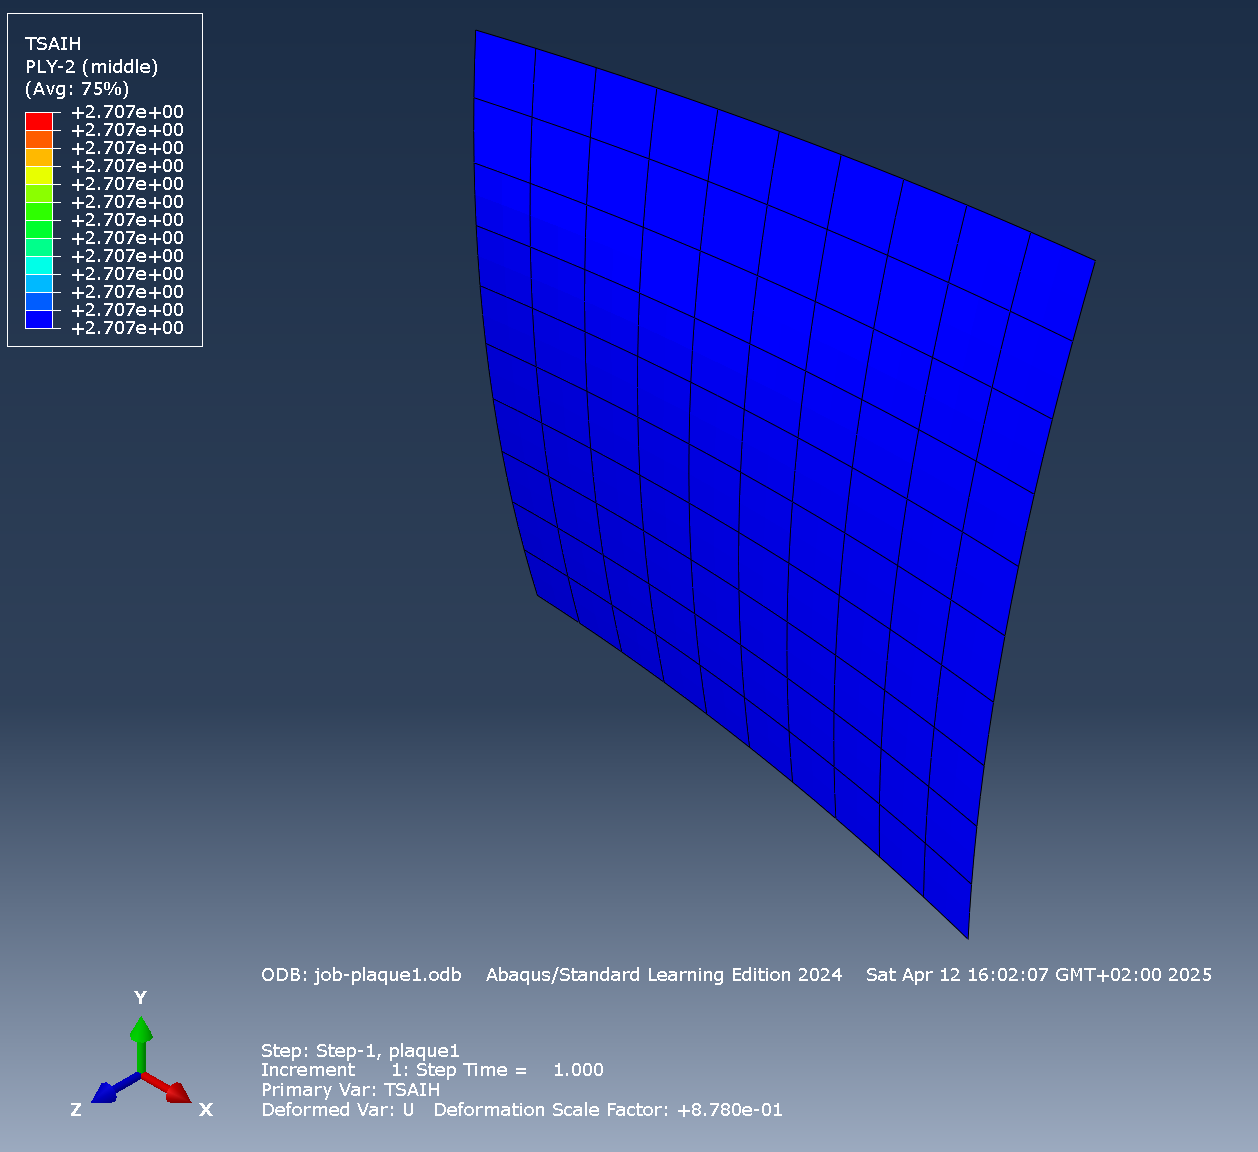
\includegraphics[width=\textwidth]{media/K_P1_L2_12042025.png} % Remplacez par le chemin de votre deuxième image
		\caption{Couche 1, plaque rectangle (William)}
		\label{fig:image2}
	\end{minipage}
\end{figure}

%résultats de la plaque 1, couche 2
\begin{figure}[h!]
	\centering
	\begin{minipage}[t][0.3\textheight]{0.495\textwidth}
		\centering
		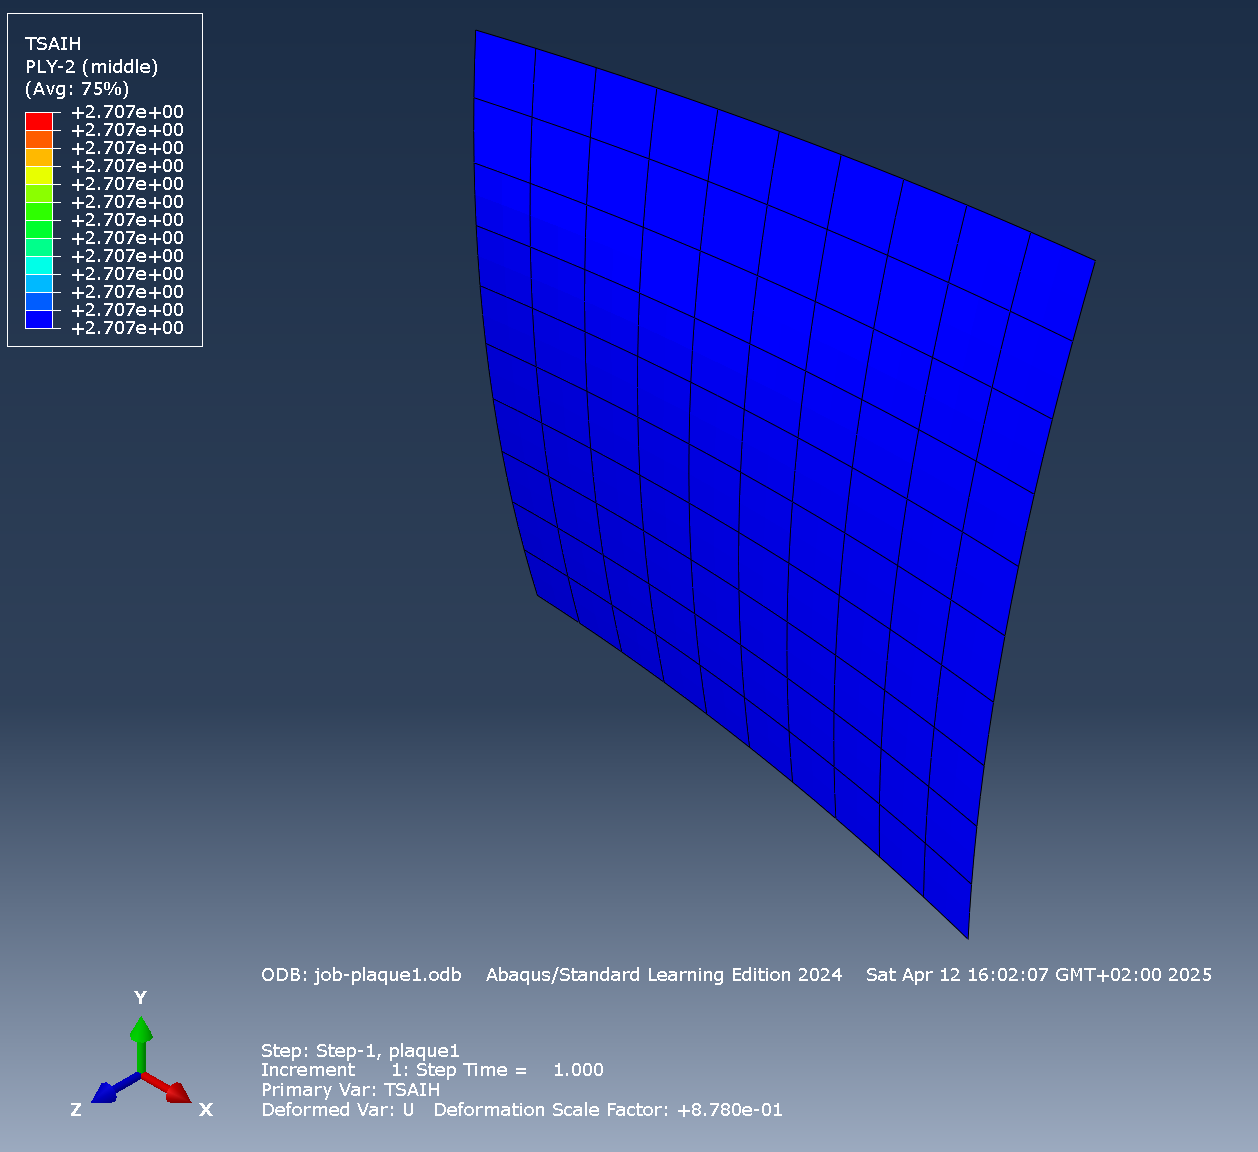
\includegraphics[width=\textwidth]{media/K_P1_L2_12042025.png} % Remplacez par le chemin de votre première image
		\caption{Couche 2, plaque carrée (Killian)}
		\label{fig:image1}
	\end{minipage}
	\hfill
	\begin{minipage}[t][0.3\textheight]{0.495\textwidth}
		\centering
		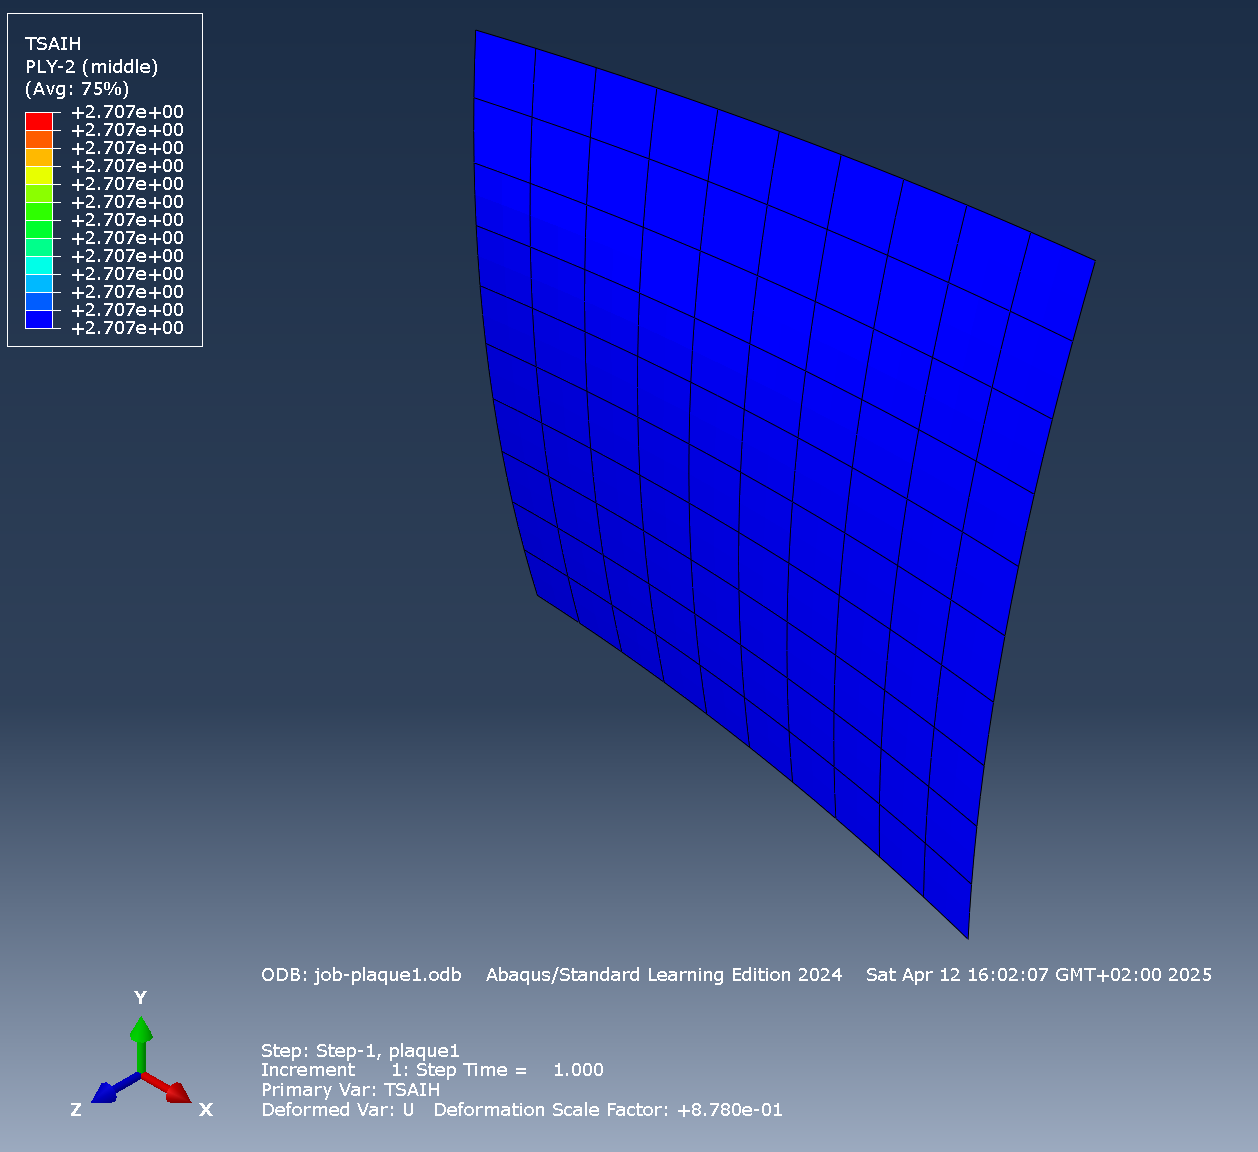
\includegraphics[width=\textwidth]{media/K_P1_L2_12042025.png} % Remplacez par le chemin de votre deuxième image
		\caption{Couche 2, plaque rectangle (William)}
		\label{fig:image2}
	\end{minipage}
\end{figure}
\clearpage

%résultats de la plaque 1, couche 3
\begin{figure}[h!]
	\centering
	\begin{minipage}{0.495\textwidth}
		\centering
		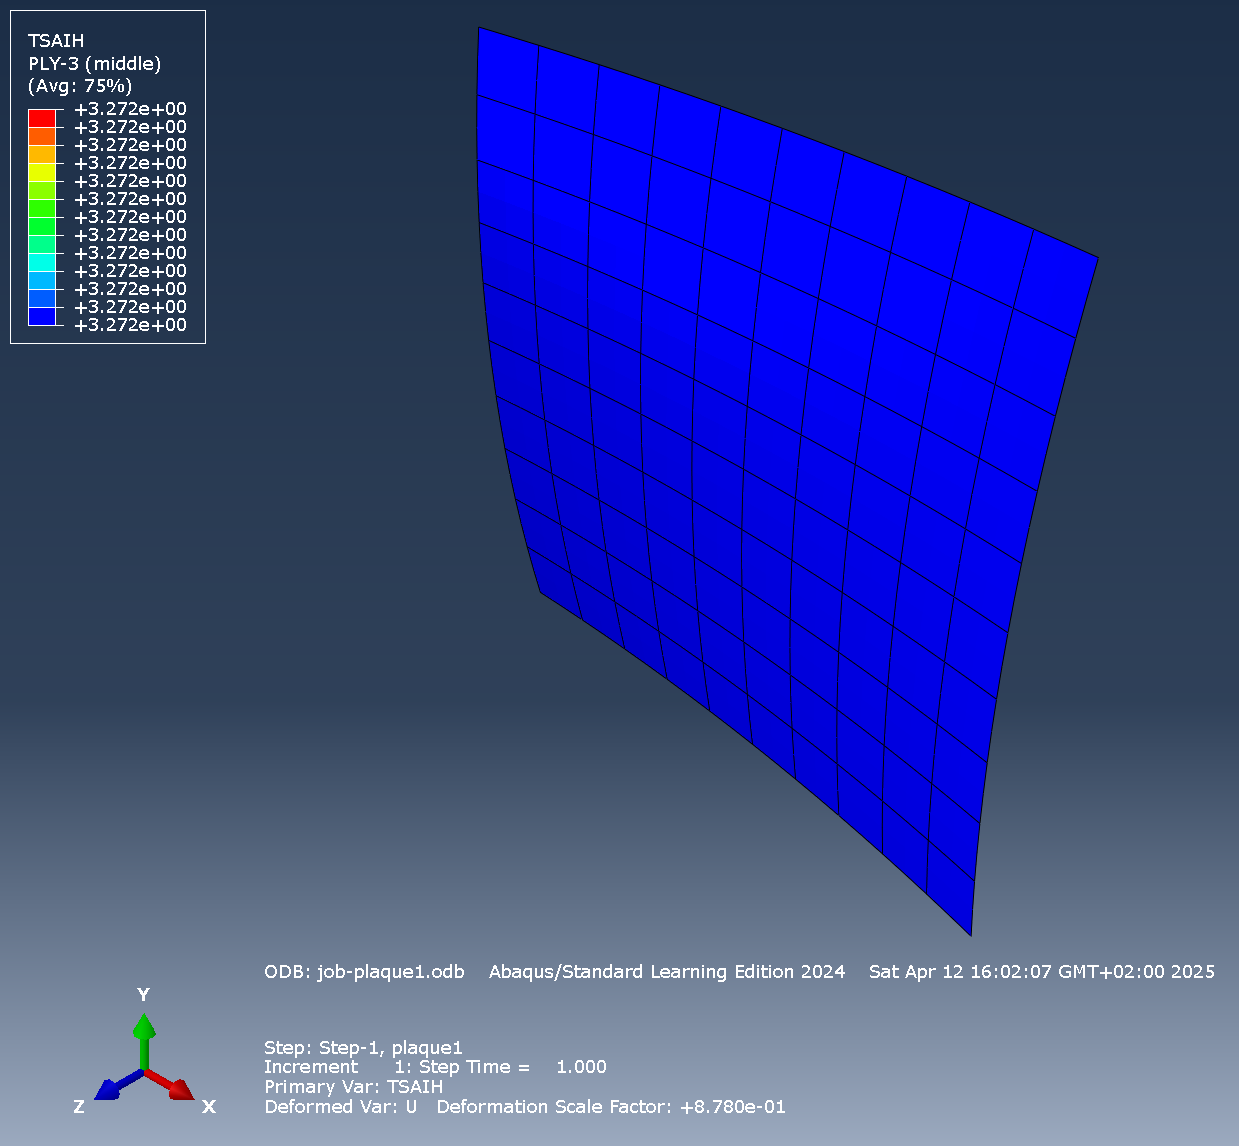
\includegraphics[width=\textwidth]{media/K_P1_L3_12042025.png} % Remplacez par le chemin de votre première image
		\caption{Couche 3, plaque carrée (Killian)}
		\label{fig:image1}
	\end{minipage}
	\hfill
	\begin{minipage}{0.495\textwidth}
		\centering
		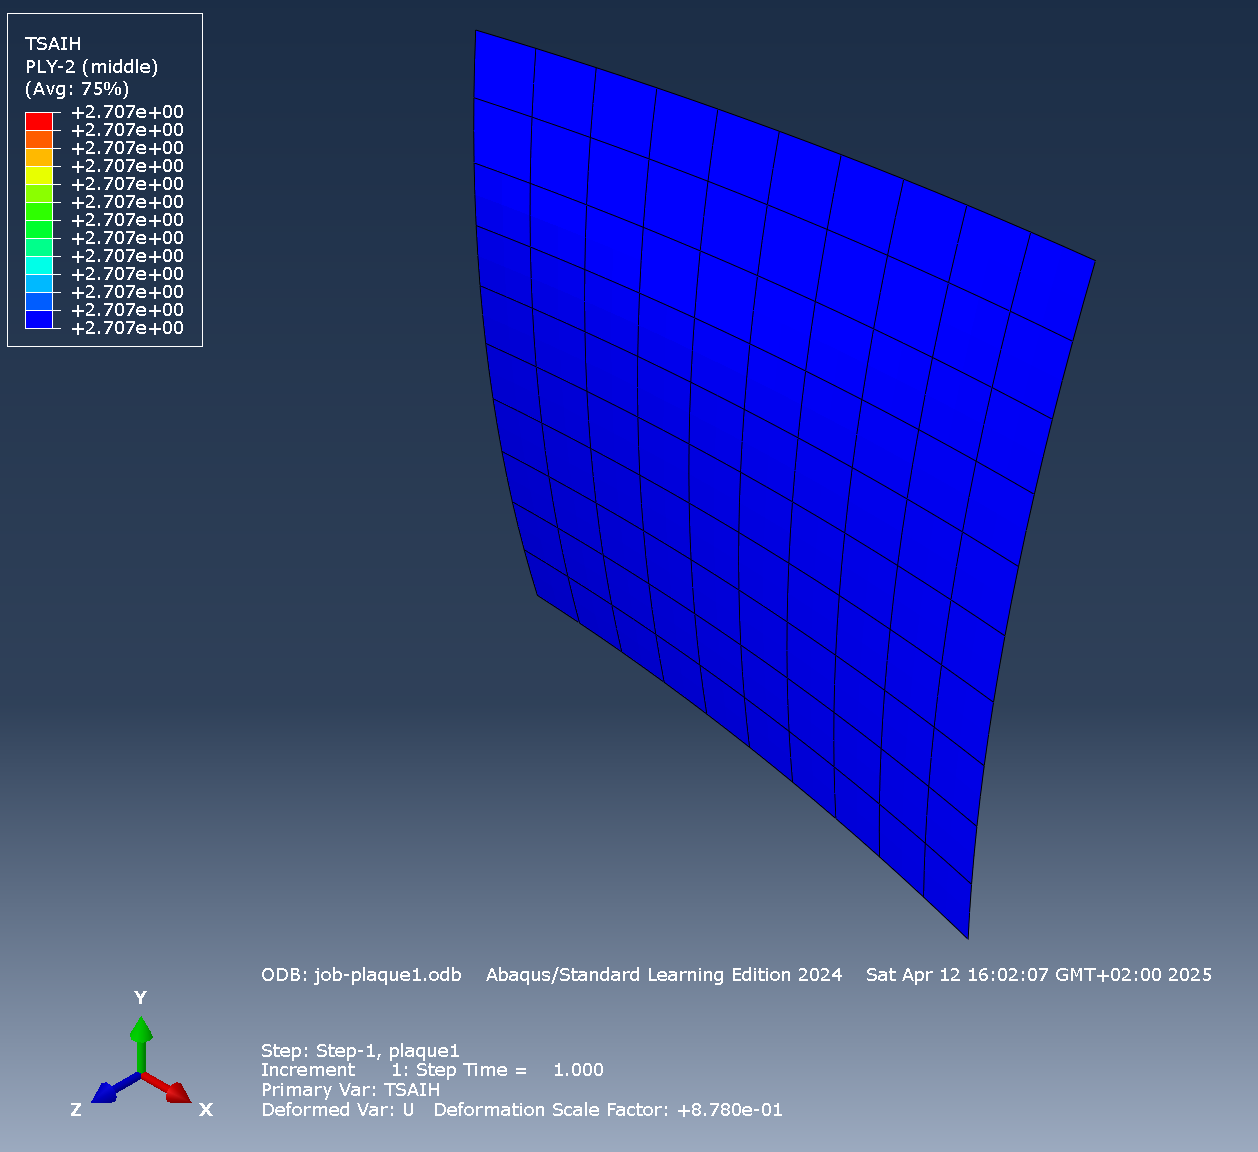
\includegraphics[width=\textwidth]{media/K_P1_L2_12042025.png} % Remplacez par le chemin de votre deuxième image
		\caption{Couche 3, plaque rectangle (William)}
		\label{fig:image2}
	\end{minipage}
\end{figure}

%résultats de la plaque 1, couche 4
\begin{figure}[h!]
	\centering
	\begin{minipage}{0.495\textwidth}
		\centering
		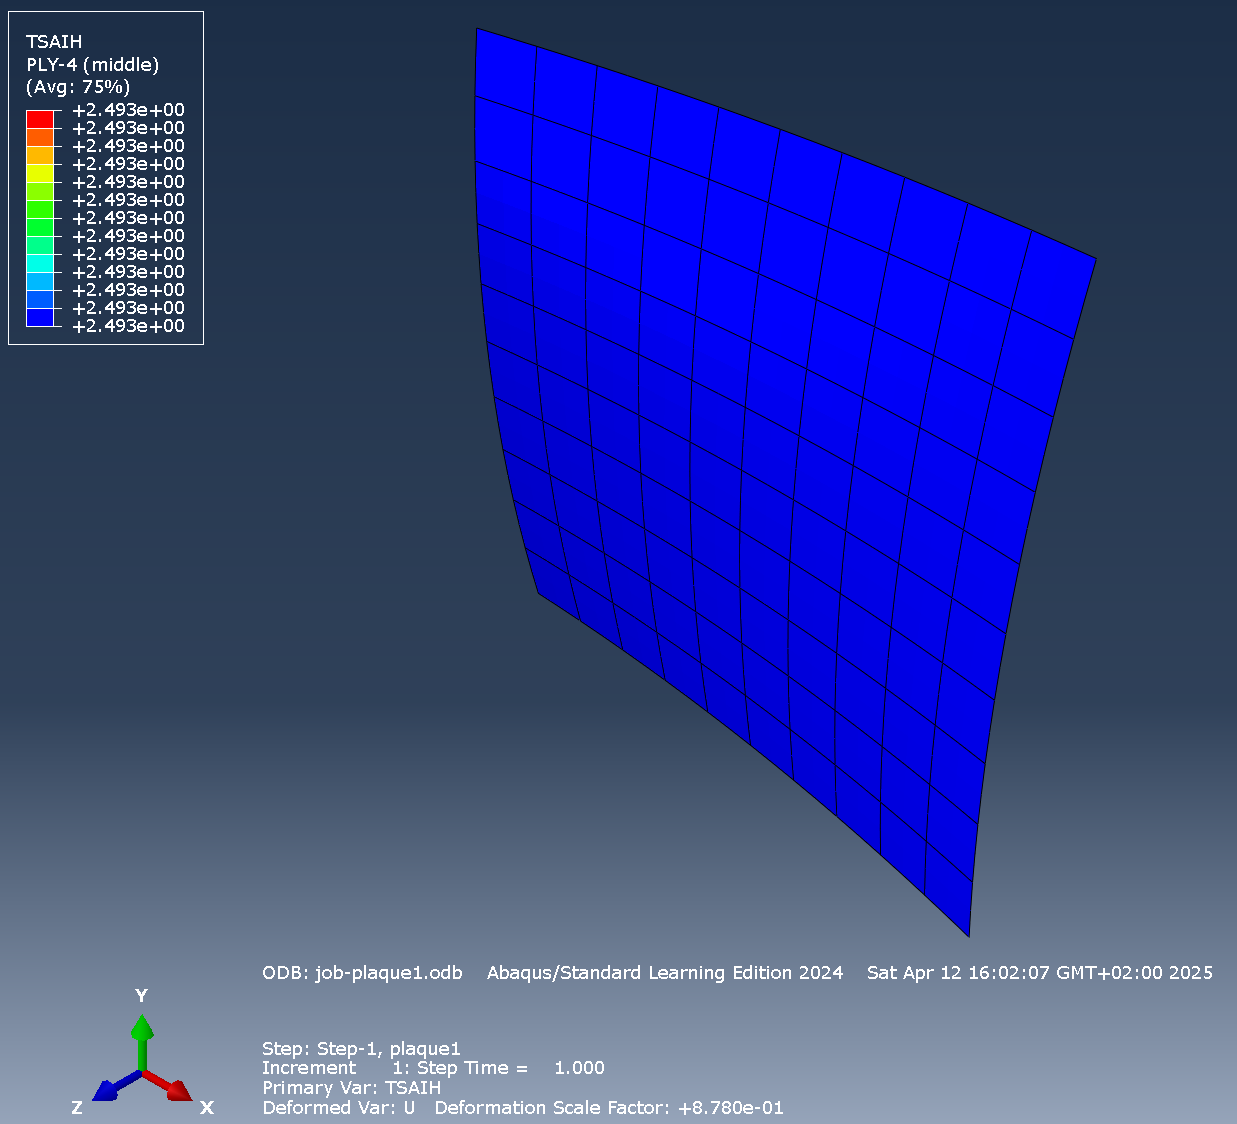
\includegraphics[width=\textwidth]{media/K_P1_L4_12042025.png} % Remplacez par le chemin de votre première image
		\caption{Couche 4, plaque carrée (Killian)}
		\label{fig:image1}
	\end{minipage}
	\hfill
	\begin{minipage}{0.495\textwidth}
		\centering
		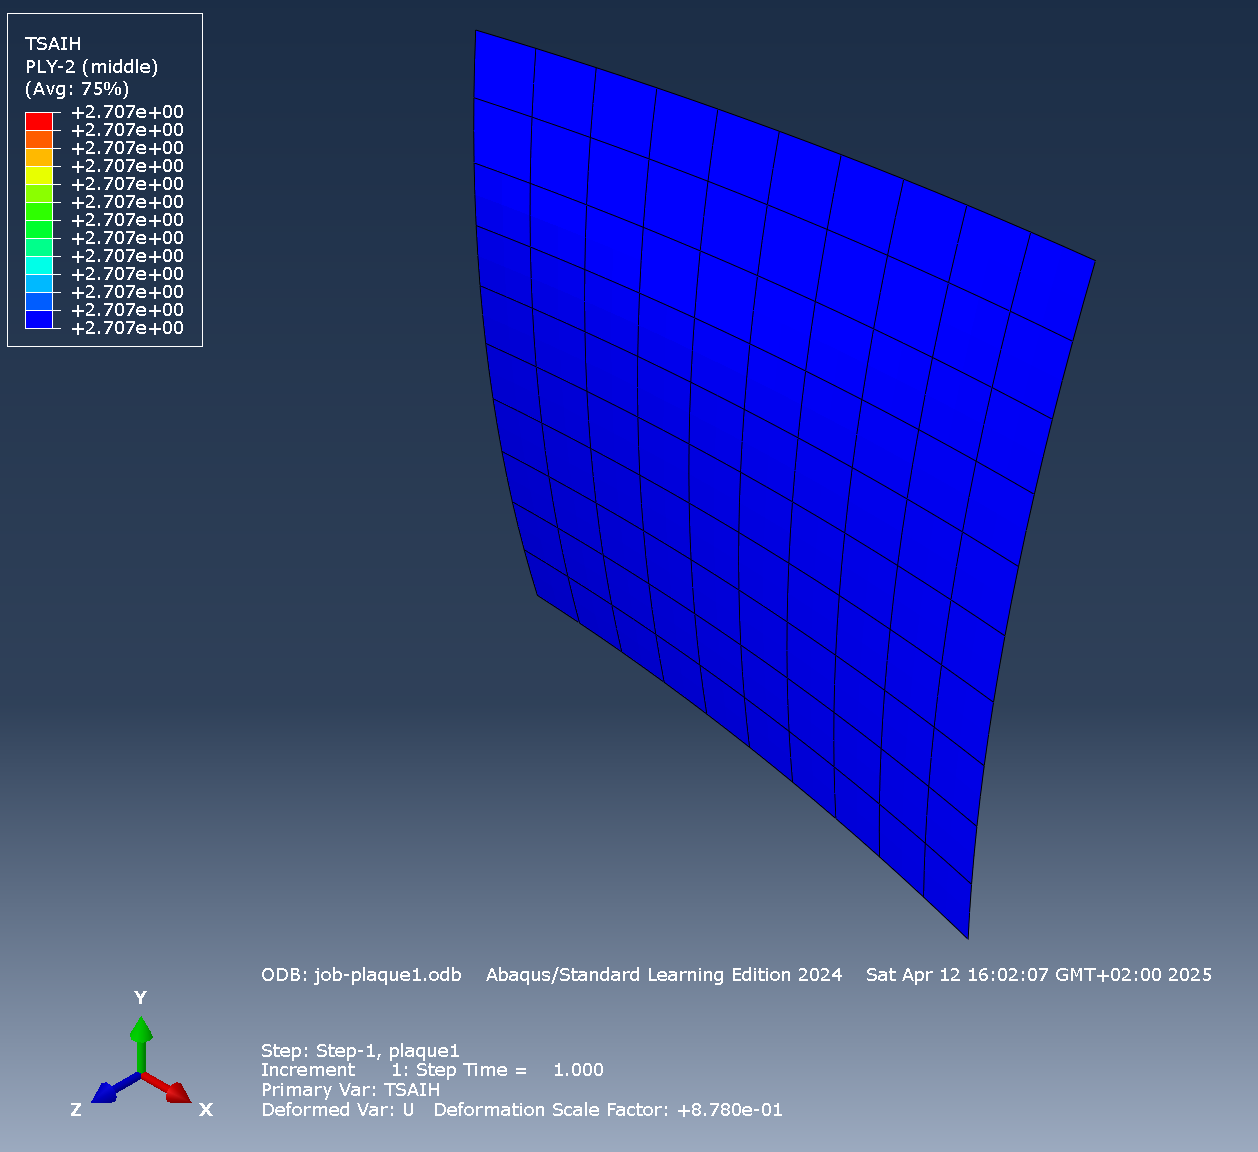
\includegraphics[width=\textwidth]{media/K_P1_L2_12042025.png} % Remplacez par le chemin de votre deuxième image
		\caption{Couche 4, plaque rectangle (William)}
		\label{fig:image2}
	\end{minipage}
\end{figure}





\section{Résultats obtenus avec la calculatrice composite sous Tableur}
Dans cette section, introduisez le sujet du TP, les objectifs et le contexte.

% Résultats
\section{Résultats}
\subsection{Exemple d'image avec légende}
\begin{figure}[h!]
	\centering
	
\includegraphics[width=0.7\textwidth]{media/logo-enit-2454399073.png} % Remplacez par le chemin de votre image
	\caption{Exemple de légende pour une image.}
	\label{fig:exemple_image}
\end{figure}

\subsection{Exemple de tableau}
\begin{table}[h!]
	\centering
	\begin{tabular}{|c|c|c|}
		\hline
		\textbf{Paramètre} & \textbf{Valeur} & \textbf{Unité} \\
		\hline
		Exemple 1          & 10              & m/s            \\
		Exemple 2          & 20              & m/s            \\
		Exemple 3          & 30              & m/s            \\
		\hline
	\end{tabular}
	\caption{Exemple de tableau avec des données.}
	\label{tab:exemple_tableau}
\end{table}

% Discussion
\section{Discussion}
Analysez les résultats obtenus, discutez des erreurs possibles et proposez des améliorations.

% Conclusion
\section{Conclusion}
Résumé des résultats principaux et conclusion générale.

% test de corp de texte
\section{Test de corps de texte}
\lipsum[1-3] % Génère trois paragraphes de texte d'exemple

% Bibliographie
\section*{Bibliographie}
\begin{itemize}
	\item Référence 1
	\item Référence 2
\end{itemize}

\end{document}